%!TEX root=../main.tex
\section{Results}
\label{sec:love_results}

In this section we demonstrate the effectiveness and speed of KISS-GP + LOVE{}, both at computing predictive variances and also at posterior sampling.
Our goal is to show that 1) LOVE{} produces uncertainties and samples that are indistinguishable from the state-of-the-art, and 2) that LOVE{} offers substantial speed improvements.
All experiments in this section use LOVE in conjunction with KISS-GP models.
See \cref{chapter:largeexact} for results where LOVE is used with standard Gaussian processes.

In the following experiments, all LOVE{} low-rank approximations use $J=50$ Lanczos iterations and KISS-GP models use $M\!=\!10,\!000$ inducing points unless otherwise stated.
We optimize models with ADAM \cite{kingma2014adam} and a learning rate of $0.1$.
All timing experiments are performed on a GTX 1070 GPU.
Exact GPs, KISS-GP models, and LOVE are implemented in our GPyTorch software.
SGPR models are implemented in GPFlow \cite{matthews2017gpflow}.

\subsection{Predictive Variances}
\label{sec:results_variances}

We measure the accuracy and speed of LOVE + KISS-GP{} variances.
In all experiments, we compare against Exact GP ({\bf Exact}) variances (without LOVE) and standard KISS-GP variances ({\bf KISS-GP w/o LOVE}).
(Note that we do not compare predictive means, as LOVE{} only affects variance cmoputations.)
We report the scaled mean absolute error (SMAE)\footnote{
  Mean absolute error divided by the variance of $y$.
} \cite{rasmussen2006gaussian} of LOVE{} + KISS-GP variances compared against these baselines.
For each dataset, we optimize the hyperparameters of a KISS-GP model.
We then apply the same hyperparameters to each baseline model.

\begin{figure}[t!]
  \centering
  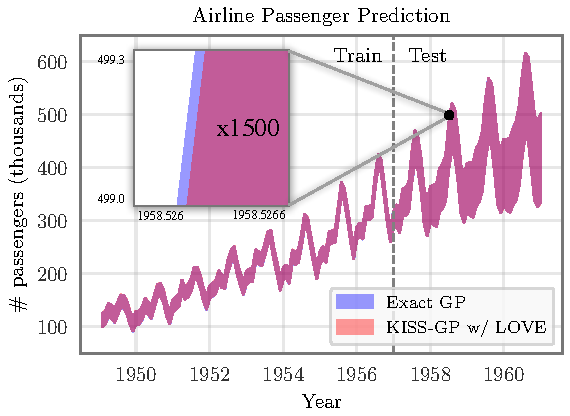
\includegraphics[width=0.65\columnwidth]{figures/airline_comparison.pdf}
  \caption[Comparison of LOVE predictive variances versus exact predictive variances on airline passenger extrapolation.]{
    Comparison of LOVE predictive variances versus exact predictive variances on airline passenger extrapolation.
    The LOVE{} variances are accurate within $10^{-4}$.
    \label{fig:airline_results}
  }
\end{figure}

\paragraph{One-dimensional example.}
We first demonstrate LOVE{} on a complex one-dimensional regression task.
The airline passenger dataset ({\bf Airline}) measures the average monthly number of passengers from 1949 to 1961 \cite{hyndman2005time}.
We aim to extrapolate the numbers for the final 4 years (48 measurements) given the first 8 years (96 measurements).
%These data exhibit short-term periodic trends as well as long-term growth trends.  Consequentially,
Accurate extrapolation on this dataset requires a kernel function capable of expressing various patterns, such as the spectral mixture (SM) kernel \cite{wilson2013gaussian}.
%Our goal is to evaluate if LOVE{} produces reliable predictive variances, even with complex kernel functions.

We compute the variances for Exact GP and KISS-GP + LOVE{} models with a $10$-mixture SM kernel.
In \cref{fig:airline_results}, we see that the LOVE + KISS-GP{} confidence intervals match the Exact GP's intervals extremely well.
The SMAE of LOVE{}'s predicted variances (compared against Exact GP variances) is $1.29 \times 10^{-4}$.
Although not shown in the plot, we confirm the reliability of these predictions by computing the log-likelihood of the test data.
We compare the LOVE + KISS-GP{} model to an Exact GP, a KISS-GP model without LOVE{}, and a sparse variational GP (SGPR) model with $M=1000$ inducing points.
All methods achieve nearly identical log-likelihoods, ranging from $-221$ to $-222$.


\begin{table}[t!]
  \caption[Speedup and accuracy of LOVE + KISS-GP{} for predictive variances.]{
    Speedup and accuracy of LOVE + KISS-GP{} for predictive variances (Deep RBF Kernels).
    Accuracy is measured by Scaled Mean Average Error.
    ($N$ is the number of data, $D$ is the dimensionality.)
    \label{tab:large_dataset_results}
  }
  \vspace{0.5ex}
  \centering
  \resizebox{\textwidth}{!}{%
    %!TEX root=../main.tex
\begin{tabular}{ |ccc||c|c||c|c| }
  \hline
  \multicolumn{3}{|c|}{\bf Dataset}
  & \multicolumn{4}{c|}{\thead{\bf Variance SMAE}}
  \\
  \cline{1-7}
  Name
  & {$N$}
  & {$D$}
  & {\thead{(vs KISS-GP w/o LOVE)}}
  & {\thead{(vs Exact GP)}}
  & {\thead{(from scratch)}}
  & {\thead{(after pre-comp.)}}
  \\
  \hhline{|===#=|=#=|=|}
  \thead{\bf Airfoil}
  & $1,\!503$
  & $6$
  & $1.30 \times 10^{-5}$
  & $7.01 \times 10^{-5}$
  & $4 \times$
  & $84 \times$
  %& $3 \times$
  %& $49 \times$
  %& $9 \times$
  %& $183 \times$
  \\

  \thead{\bf Skillcraft}
  & $3,\!338$
  & $19$
  & $2.00 \times 10^{-7}$
  & $2.86 \times 10^{-4}$
  & $25 \times$
  & $167 \times$
  %& $4 \times$
  %& $70 \times$
  %& $17 \times$
  %& $110 \times$
  \\

  \thead{\bf Parkinsons}
  & $5,\!875$
  & $20$
  & $8.80 \times 10^{-5}$
  & $5.18 \times 10^{-3}$
  & $46 \times$
  & $443 \times$
  %& $3 \times$
  %& $33 \times$
  %& $16 \times$
  %& $152 \times$
  \\

  \thead{\bf PoleTele}
  & $15,\!000$
  & $26$
  & $2.90 \times 10^{-5}$
  & $1.08 \times 10^{-3}$
  & $78 \times$
  & $1178 \times$
  %& $1.5 \times$
  %& $40 \times$
  %& $21 \times$
  %& $343 \times$
  \\

  \thead{\bf Elevators}
  & $16,\!599$
  & $18$
  & $1.20 \times 10^{-6}$
  & --
  & $64 \times$
  & $1017 \times$
  %& $2 \times$
  %& $31 \times$
  %& $20 \times$
  %& $316 \times$
  \\

  \thead{\bf Kin40k}
  & $40,\!000$
  & $8$
  & $3.90 \times 10^{-7}$
  & --
  & $31 \times$
  & $2065 \times$
  %& $8 \times$
  %& $81 \times$
  %& $12 \times$
  %& $798 \times$
  \\

  \thead{\bf Protein}
  & $45,\!730$
  & $9$
  & $5.30 \times 10^{-5}$
  & --
  & $44 \times$
  & $1151 \times$
  %& $10 \times$
  %& $109 \times$
  %& $20 \times$
  %& $520 \times$
  \\
  \hline
\end{tabular}

  }
  \vspace{1em}

  \resizebox{\textwidth}{!}{%
    %!TEX root=../main.tex
\begin{tabular}{ |ccc||c|c|c|c| }
  \hline
  \multicolumn{3}{|c||}{\bf Dataset}
  & \multicolumn{4}{c|}{\thead{\bf Speedup over SGPR}}
  \\
  \cline{1-7}
  \multirow{2}{*}{Name}
  & \multirow{2}{*}{$N$}
  & \multirow{2}{*}{$D$}
  & \thead{(from scratch)}
  & \thead{(after pre-comp.)}
  & \thead{(from scratch)}
  & \thead{(after pre-comp.)}
  \\
   &  &  & $M=100$ & $M=100$ & $M=1000$ & $M=1000$
  \\
  \hhline{|===#=|=|=|=|}
  \thead{\bf Airfoil}
  & $1,\!503$
  & $6$
  %& $1.30 \times 10^{-5}$
  %& $7.01 \times 10^{-5}$
  %& $4 \times$
  %& $84 \times$
  & $3 \times$
  & $49 \times$
  & $9 \times$
  & $183 \times$
  \\

  \thead{\bf Skillcraft}
  & $3,\!338$
  & $19$
  %& $2.00 \times 10^{-7}$
  %& $2.86 \times 10^{-4}$
  %& $25 \times$
  %& $167 \times$
  & $4 \times$
  & $70 \times$
  & $17 \times$
  & $110 \times$
  \\

  \thead{\bf Parkinsons}
  & $5,\!875$
  & $20$
  %& $8.80 \times 10^{-5}$
  %& $5.18 \times 10^{-3}$
  %& $46 \times$
  %& $443 \times$
  & $3 \times$
  & $33 \times$
  & $16 \times$
  & $152 \times$
  \\

  \thead{\bf PoleTele}
  & $15,\!000$
  & $26$
  %& $2.90 \times 10^{-5}$
  %& $1.08 \times 10^{-3}$
  %& $78 \times$
  %& $1178 \times$
  & $1.5 \times$
  & $40 \times$
  & $21 \times$
  & $343 \times$
  \\

  \thead{\bf Elevators}
  & $16,\!599$
  & $18$
  %& $1.20 \times 10^{-6}$
  %& --
  %& $64 \times$
  %& $1017 \times$
  & $2 \times$
  & $31 \times$
  & $20 \times$
  & $316 \times$
  \\

  \thead{\bf Kin40k}
  & $40,\!000$
  & $8$
  %& $3.90 \times 10^{-7}$
  %& --
  %& $31 \times$
  %& $2065 \times$
  & $8 \times$
  & $81 \times$
  & $12 \times$
  & $798 \times$
  \\

  \thead{\bf Protein}
  & $45,\!730$
  & $9$
  %& $5.30 \times 10^{-5}$
  %& --
  %& $44 \times$
  %& $1151 \times$
  & $10 \times$
  & $109 \times$
  & $20 \times$
  & $520 \times$
  \\
  \hline
\end{tabular}

  }
\end{table}

\paragraph{Large datasets.}
We measure the accuracy of LOVE{} variances on several large-scale regression benchmarks from the UCI repository \cite{asuncion2007uci}.
%We compute the variance for all test set data points.
Each of the models use deep RBF kernels (DKL) with the architectures described in \cite{wilson2016deep}.
%Deep RBF kernels are extremely flexible (with up to $10^5$ hyperparameters) and are well suited to model many types of functions.
In \cref{tab:large_dataset_results}, we report the SMAE of the LOVE + KISS-GP{} variances compared against the two baselines.
On all datasets, we find that LOVE{} matches KISS-GP w/o LOVE{} to at least $5$ decimal places.
Furthermore, LOVE + KISS-GP{} is able to approximate Exact variances with no more than than $10^{-3}$ error.
For any given test point, the maximum variance error is similarly small (e.g. $\leq \! 2.6\%$ on Skillcraft and $\leq \! 2.0\%$ on PoleTele).
Therefore, using LOVE{} to compute variances results in \emph{almost no loss in accuracy}.

\paragraph{Speedup.}
In \cref{tab:large_dataset_results} we compare the variance computation speed of a KISS-GP model with and without LOVE{} on the UCI datasets.
In addition, we compare against SGPR models (with non-deep RBF kernels), a competitive scalable GP approach.
On all datasets, we measure the time to compute variances {\bf from scratch}, which includes the cost of pre-computation.
In addition, we report the speed {\bf after pre-computing} any terms that aren't specific to test points.
We see in \cref{tab:large_dataset_results} that KISS-GP + LOVE{} yields a substantial speedup over KISS-GP without LOVE{}.
The speedup is between $4\times$ and $44\times$, even when accounting for LOVE{}'s precomputation.
At test time after pre-computation, LOVE{} is \emph{up to $2,\!000\times$ faster}.
Additionally, LOVE + KISS-GP{} is significantly faster than SGPR models.
For SGPR models with $M=100$ inducing points, the LOVE + KISS-GP{} model (with $M=10,\!000$ inducing points) is up to $10\times$ faster before pre-computation and $100\times$ faster after.
With $M=1000$ SGPR models, LOVE + KISS-GP{} is up to $20\times$/$500\times$ faster before/after precomputation.
The biggest improvements are obtained on the largest datasets since LOVE{}, unlike other methods, is independent of dataset size at test time.

\begin{figure}[t!]
  \centering
  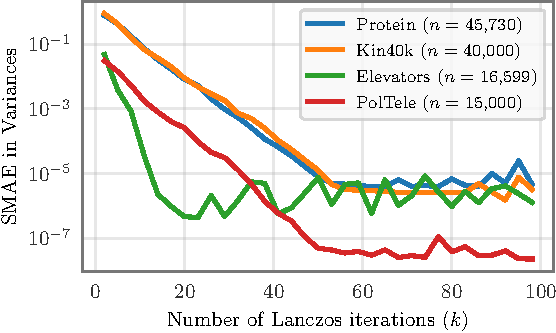
\includegraphics[width=0.65\columnwidth]{figures/lanczos_accuracy.pdf}
  \vspace{-2ex}
  \caption[LOVE variance error versus number of Lanczos iterations.]{
    LOVE variance error versus number of Lanczos iterations
    (KISS-GP model, $M=10,\!000$. Protein, Kin40k, PoleTele, and Elevators UCI datasets).
    \label{fig:lanczos_accuracy}
  }
  \vspace{-1ex}
\end{figure}

\paragraph{Accuracy vs. Lanczos iterations.}
In \cref{fig:lanczos_accuracy}, we measure the accuracy of LOVE{} as a function of the number of Lanczos iterations ($J$), which corresponds to the rank of the $\blue \widetilde \bR$ matrix in \cref{eqn:pred_covar_ski_fast}.
We train a KISS-GP model with a deep RBF kernel on the four largest datasets from \cref{tab:large_dataset_results}, measuring the SMAE of LOVE + KISS-GP's predictive variances.\footnote{
  As measured against the variances from KISS-GP w/o LOVE.
}
As seen in \cref{fig:lanczos_accuracy}, error decreases \emph{exponentially} with the number of Lanczos iterations, up until roughly $50$ iterations.
After roughly $50$ iterations, the error levels off, though this may be an artifact of floating-point precision (which may also cause small subsequent fluctuations).



\subsection{Sampling}

\begin{table}[t!]
  \caption[Accuracy and computation time of drawing samples from the posterior distribution.]{
    Accuracy and computation time of drawing samples from the predictive distribution.
    \label{tab:sampling_results}
  }
  \vspace{0.5ex}
  \centering
  \resizebox{\textwidth}{!}{%
    %!TEX root=../main.tex
\begin{tabular}{ |c||c|c|c|c|c| }
  \hline
  \multirow{4}{*}{\thead{\bf Dataset} }
  & \multicolumn{5}{c|}{\thead{\bf Sample Covariance Error} }

  \\
  \cline{2-6}


  & \thead{\bf Exact GP \\ \bf w/ Cholesky}
  & \thead{\bf Fourier \\ \bf Features}
  & \thead{\bf SGPR \\ ($M=100$)}
  & \thead{\bf SGPR \\ ($M=1000$)}
  & \thead{\bf LOVE \\ \bf + KISS-GP}
  %& \thead{\bf Fourier \\ \bf Features}
  %& \thead{\bf SGPR (m=100)}
  %& \thead{\bf SGPR (m=1000)}
  %& \thead{\bf KISS-GP \\ \bf w/ LOVE{} \\ (from scratch)}
  %& \thead{\bf KISS-GP \\ \bf w/ LOVE{} \\ (after pre-comp.)}
  \\
  \hhline{|=#=|=|=|=|=|}

  \thead{\bf PolTele}
  & $\mathbf{8.8 \times 10^{-4}}$
  & $1.8 \times 10^{-3}$
  & $4.9 \times 10^{-3}$
  & $2.7 \times 10^{-3}$
  & $\mathbf{7.5 \times 10^{-4}}$
  %& $22 \times$
  %& $24 \times$
  %& $3 \times$
  %& $21 \times$
  %& $\mathbf{881 \times}$
  \\

  \thead{\bf Elevators}
  & $\mathbf{2.6 \times 10^{-7}}$
  & $3.1 \times 10^{-4}$
  & $8.7 \times 10^{-6}$
  & $3.6 \times 10^{-6}$
  & $\mathbf{5.5 \times 10^{-7}}$
  %& $31 \times$
  %& $33 \times$
  %& $4 \times$
  %& $25 \times$
  %& $\mathbf{1062 \times}$
  \\
  \hline

  \thead{\bf BO (Eggholder)}
  & $\mathbf{7.7 \times 10^{-4}}$
  & $1.5 \times 10^{-3}$
  & $\mathbf{8.1 \times 10^{-4}}$
  & --
  & $\mathbf{8.0 \times 10^{-5}}$
  %& $16 \times$
  %& $8 \times$
  %& --
  %& $19 \times$
  %& $\mathbf{775 \times}$
  \\

  \thead{\bf BO (Styblinski-Tang)}
  & $\mathbf{5.4 \times 10^{-4}}$
  & $7.3 \times 10^{-3}$
  & $\mathbf{5.2 \times 10^{-4}}$
  & --
  & $\mathbf{5.2 \times 10^{-4}}$
  %& $11 \times$
  %& $8 \times$
  %& --
  %& $42 \times$
  %& $\mathbf{18,\!100 \times}$
  \\
  \hline

\end{tabular}

  }
  \vspace{1em}

  \resizebox{\textwidth}{!}{%
    %!TEX root=../main.tex
\begin{tabular}{ |c||c|c|c|c|c| }
  \hline
  \multirow{4}{*}{\thead{\bf Dataset} }
  & \multicolumn{5}{c|}{\thead{\bf Speedup over Exact GP w/ Cholesky} }

  \\
  \cline{2-6}


  %& \thead{\bf Exact GP \\ \bf w/ Cholesky}
  %& \thead{\bf Fourier \\ \bf Features}
  %& \thead{\bf SGPR (m=100)}
  %& \thead{\bf SGPR (m=1000)}
  %& \thead{\bf KISS-GP \\ \bf w/ LOVE}
  & \thead{\bf Fourier \\ \bf Features}
  & \thead{\bf SGPR \\ ($M=100$)}
  & \thead{\bf SGPR \\ ($M=1000$)}
  & \thead{\bf LOVE \\ \bf + KISS-GP{} \\ (from scratch)}
  & \thead{\bf LOVE \\ \bf + KISS-GP{} \\ (after pre-comp.)}
  \\
  \hhline{|=#=|=|=|=|=|}

  \thead{\bf PolTele}
  %& $\mathbf{8.8 \times 10^{-4}}$
  %& $1.8 \times 10^{-3}$
  %& $4.9 \times 10^{-3}$
  %& $2.7 \times 10^{-3}$
  %& $\mathbf{7.5 \times 10^{-4}}$
  & $22 \times$
  & $24 \times$
  & $3 \times$
  & $21 \times$
  & $\mathbf{881 \times}$
  \\

  \thead{\bf Elevators}
  %& $\mathbf{2.6 \times 10^{-7}}$
  %& $3.1 \times 10^{-4}$
  %& $8.7 \times 10^{-6}$
  %& $3.6 \times 10^{-6}$
  %& $\mathbf{5.5 \times 10^{-7}}$
  & $31 \times$
  & $33 \times$
  & $4 \times$
  & $25 \times$
  & $\mathbf{1062 \times}$
  \\
  \hline

  \thead{\bf BO (Eggholder)}
  %& $\mathbf{7.7 \times 10^{-4}}$
  %& $1.5 \times 10^{-3}$
  %& $\mathbf{8.1 \times 10^{-4}}$
  %& --
  %& $\mathbf{8.0 \times 10^{-5}}$
  & $16 \times$
  & $8 \times$
  & --
  & $19 \times$
  & $\mathbf{775 \times}$
  \\

  \thead{\bf BO (Styblinski-Tang)}
  %& $\mathbf{5.4 \times 10^{-4}}$
  %& $7.3 \times 10^{-3}$
  %& $\mathbf{5.2 \times 10^{-4}}$
  %& --
  %& $\mathbf{5.2 \times 10^{-4}}$
  & $11 \times$
  & $8 \times$
  & --
  & $42 \times$
  & $\mathbf{18,\!100 \times}$
  \\
  \hline

\end{tabular}

  }
\end{table}

We evaluate the quality of posterior samples drawn with LOVE + KISS-GP{} as described in \cref{sec:sampling_method}.
We compare against three baselines: sampling from an {\bf Exact GP} using the Cholesky decomposition, sampling from an {\bf SGPR} model with Cholesky, and sampling an exact GP with random {\bf Fourier features} \citep{rahimi2008random}.
%The LOVE + KISS-GP{} and SGPR models use the same architecture as described in the previous section.
For Fourier features, we use 5000 random features---the maximum number of features without exhausting available GPU memory.
The model hyperparameters are learned on an Exact GP and then shared across all baselines.
We use two UCI datasets (PolTele and Eleveators) datasets as well as two Bayesian optimization benchmark functions (Eggholder: 2 dimensional, and Styblinski-Tang: 10 dimensional).
For the BayesOpt functions, we evaluate the model after 100 queries of max value entropy search \cite{wang2017max}.
For Eggholder, we use a standard (non-deep) RBF kernel;  for Syblinski-Tang we use the additive kernel suggested by~\citet{kandasamy2015high}.\footnote{
  The Syblinski-Tang KISS-GP model uses the sum of 10 RBF kernels---one for each dimension---and $M=100$ inducing points.
}

\paragraph{Sampling accuracy.}
In \cref{tab:sampling_results} we evaluate the accuracy of the different sampling methods.
We draw $S\!=\!1000$ samples at $T\!=\!10,\!000$ test locations and compare the empirical covariance matrix with the true posterior covariance.
The reported numbers are element-wise mean absolute errors.
It is worth noting that all methods incur some sampling error---even when sampling with an Exact GP.
Nevertheless, Exact GPs, SGPR, and LOVE{} produce very accurate sample covariance matrices.
In particular, Exact GPs and LOVE{} achieve between 1 and 3 orders of magnitude less error than the random Fourier Feature method.

\paragraph{Speed.}
Though LOVE{}, Exact GPs, and SGPR have similar accuracies, LOVE{} is much faster.
Even when accounting for LOVE's pre-computation time (i.e. sampling ``from scratch''), LOVE{} is comparable to Fourier features and SGPR in terms of speed.
At test time (i.e. after pre-computation), LOVE{} is up to $18,\!000$ times faster than Exact.

\paragraph{Bayesian optimization.}
Many acquisition functions in Bayesian optimization rely on sampling from the GP posterior.
For example, max-value entropy search \cite{wang2017max} uses samples to estimate the function's maximum value $p(y_\text{max} \! \mid \! \dset)$.
%
\begin{figure}[t!]
  \centering
  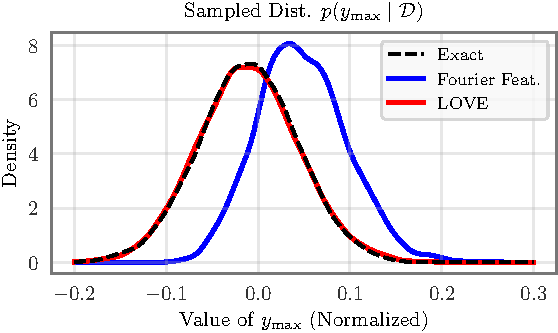
\includegraphics[width=0.65\columnwidth]{figures/love_sampling_comparison.pdf}
  \caption[Comparison of LOVE and Random Fourier Features for BayesOpt sampling.]{
    Comparison of LOVE and Random Fourier Features for BayesOpt sampling.
    Each line represents an approximation of maximum value distribution $p(y_\text{max} \mid \dset)$ using different sampling methods (exact sampling, Random Fourier Features, and LOVE + KISS-GP).
    Samples drawn with LOVE+KISSGP closely match samples drawn using an Exact GP.
    (Dataset: (normalized) Eggholder function after 100 iterations of BayesOpt.)
    \label{fig:love_sampling_comparison}
  }
\end{figure}
%
In \cref{fig:love_sampling_comparison}, we visualize each method's sampled distribution of $p(y_\text{max} \! \mid \! \dset)$ for the Eggholder function.
We plot kernel density estimates of this distribution after $100$ BayesOpt iterations.\footnote{
  Using the max-value entropy search acquisition function \citep{wang2017max}.
}
Since the Exact GP sampling method uses the Cholesky decomposition, its sampled max-value distribution can be considered closest to ground truth.
The Fourier feature distribution differs significantly from the Exact GP distribution.
In contrast, LOVE{} very closely resembles Exact GPs, yet can be computed up to $700 \times$ faster (\cref{tab:sampling_results}).
